\documentclass[12pt]{article}

\usepackage{amsmath,amsthm,amsfonts,amssymb,amsxtra}
\usepackage{tikz,array}
\usetikzlibrary{arrows}
\renewcommand{\theenumi}{(\alph{enumi})} 
\renewcommand{\labelenumi}{\theenumi}

\pagestyle{empty}
\setlength{\textwidth}{7in}
\setlength{\oddsidemargin}{-0.5in}
\setlength{\topmargin}{-1.0in}
\setlength{\textheight}{9.5in}

\theoremstyle{definition}
\newtheorem{problem}{Problem}

\begin{document}

\noindent{\large\bf MATH 242}\hfill{\large\bf Test\#3}\hfill{\large\bf
  Spring 2018}\hfill{\large\bf Page 1/6}\hrule

\bigskip
\begin{center}
  \begin{tabular}{|ll|}
    \hline & \cr
    {\bf Name: } & \makebox[12cm]{\hrulefill}\cr & \cr
    {\bf VIP ID:} & \makebox[12cm]{\hrulefill}\cr & \cr
    \hline
  \end{tabular}
\end{center}
\begin{itemize}
\item Write your name and your VIP ID in the space provided above.
\item The test has six (6) pages, including this one and a formula sheet at the end.
\item \textbf{Do not detach} the formula sheet from the booklet.
\item Show sufficient work to justify all answers unless otherwise stated in the problem.  Correct answers with inconsistent work may not be given credit.
\item Credit for each problem is given at the right of each problem number.
\end{itemize}
\hrule

\begin{center}
  \begin{tabular}{|c|c|c|}
    \hline
    &&\cr
    {\large\bf Page} & {\large\bf Max} & {\large\bf Points} \cr
    &&\cr
    \hline
    &&\cr
    {\Large 2} & \Large 20 & \cr
    &&\cr
    \hline
    &&\cr
    {\Large 3} & \Large 30 & \cr
    &&\cr
    \hline
    &&\cr
    {\Large 4} & \Large 30 & \cr
    &&\cr
    \hline
    &&\cr
    {\Large 5} & \Large 20 & \cr
    &&\cr
    \hline\hline
    &&\cr
    {\large\bf Total} & \Large 100 & \cr
    &&\cr
    \hline
  \end{tabular}
\end{center}
\newpage

%%%%%%%%%%%%%%%%%%%%%%%%%%%%%%%%%%%%% Page 2
\noindent{\large\bf MATH 242}\hfill{\large\bf Test\#3}\hfill{\large\bf Spring 2018}\hfill{\large\bf Page 2/6}\hrule

\bigskip
\begin{problem}[10 pts]
Suppose that the population $P(t)$ of a country after $t$ years satisfies the differential equation.  
\begin{equation*}
\frac{dP}{dt} = kP(200-P)
\end{equation*}
with $k$ constant.  Its population in 1940 was 100 million and was then growing at the rate of 1 million per year.  Predict this country's population in the year 2020.
\vspace{6cm}
\begin{flushright}
\begin{tikzpicture}
\draw (-2cm, 0.5cm) node{Population in 2020:};
\draw (0cm,-0.2cm) rectangle (5cm,1.2cm);
\end{tikzpicture}
\end{flushright}
\end{problem} 
\hrule

\begin{problem}[10 pts]
Plot a slope field to indicate the stability of the following population model:
\begin{equation*}
\frac{dP}{dt} = (P-2)^2(P-4)^3(2P^2-13P+21)
\end{equation*}
\end{problem}

\newpage

%%%%%%%%%%%%%%%%%%%%%%%%%%%%%%%%%%%%% Page 3
\noindent{\large\bf MATH 242}\hfill{\large\bf Test\#3}\hfill{\large\bf
  Spring 2018}\hfill{\large\bf Page 3/6}\hrule

\bigskip
\begin{problem}[20 pts---10 pts each part]
During the period from 1790 to 1930, the U.S.~population $P(t)$ after $t$ years grew from 3.9 million to 123.2 million.  Throughout this period, $P(t)$ remained close to the solution of the initial value problem
\begin{equation*}
\frac{dP}{dt} = 0.03135 P - 0.0001489 P^2, \quad P(0) = 3.9.
\end{equation*}
\begin{enumerate}
  \item What limiting population does it predict?
  \vspace{0.5cm}
  \begin{flushright}
  \begin{tikzpicture}
  \draw (0cm,-0.2cm) rectangle (3cm,1.2cm);
  \end{tikzpicture}
  \end{flushright}
  \item What 1930 population does this model predict?
  \vspace{4cm}
  \begin{flushright}
  \begin{tikzpicture}
  \draw (0cm,-0.2cm) rectangle (3cm,1.2cm);
  \end{tikzpicture}
  \end{flushright}
\end{enumerate}
\end{problem}
\hrule

\begin{problem}[10 pts]
Consider a logistic population $P(t)$ of fish on a lake, measured in hundreds after $t$ years, with $k=3$ and $M=6$.  Suppose that 450 fish are \emph{harvested} annually (at a constant rate throughout the year).  If the lake is initially stocked with 375 fish, when will its population reach 90\% of the carrying capacity?
\vspace{5cm}
\begin{flushright}
  \begin{tikzpicture}
  \draw (0cm,-0.2cm) rectangle (3cm,1.2cm);
  \end{tikzpicture}
  \end{flushright}
\end{problem}

\newpage

%%%%%%%%%%%%%%%%%%%%%%%%%%%%%%%%%%%%% Page 4
\noindent{\large\bf MATH 242}\hfill{\large\bf Test\#3}\hfill{\large\bf
  Spring 2018}\hfill{\large\bf Page 4/6}\hrule

\bigskip
\begin{problem}[10 pts]
Find the family of curves for which the length of the part of the tangent between the point of contact $(x,y)$ and the $y$--axis is equal to half the $y$--intercept of the tangent.
\vspace{4cm}
\begin{flushright}
\begin{tikzpicture}
\draw (0cm,-0.2cm) rectangle (5cm,1.2cm);
\end{tikzpicture}
\end{flushright}
\end{problem}
\hrule

\begin{problem}[20 pts---10 pts each]
Find the orthogonal trajectories of each of the following families of curves:
\begin{enumerate}
  \item $3x^2+5y^2 = k$
  \vspace{4cm}
  \begin{flushright}
  \begin{tikzpicture}
  \draw (0cm,-0.2cm) rectangle (5cm,1.2cm);
  \end{tikzpicture}
  \end{flushright}
  \item $y^2 = 3x^2(2-kx)$
  \vspace{4cm}
  \begin{flushright}
  \begin{tikzpicture}
  \draw (0cm,-0.2cm) rectangle (5cm,1.2cm);
  \end{tikzpicture}
  \end{flushright}
\end{enumerate}
\end{problem}

\newpage

%%%%%%%%%%%%%%%%%%%%%%%%%%%%%%%%%%%%% Page 5
\noindent{\large\bf MATH 242}\hfill{\large\bf Test\#3}\hfill{\large\bf
  Spring 2018}\hfill{\large\bf Page 5/6}\hrule

\bigskip
\begin{problem}[10 pts]
Find all curves for which the subtangent at any point $(x,y)$ is equal to one third of the square of the abscissa.
\vspace{8cm}
\begin{flushright}
  \begin{tikzpicture}
  \draw (0cm,-0.2cm) rectangle (5cm,1.2cm);
  \end{tikzpicture}
  \end{flushright}
\end{problem}
\hrule
\begin{problem}[10 pts]
Find all curves for which the normal at point $(x,y)$ and the line joining the origin with that point form an isosceles triangle having its base on the $x$--axis.
\vspace{9cm}
\begin{flushright}
  \begin{tikzpicture}
  \draw (0cm,-0.2cm) rectangle (5cm,1.2cm);
  \end{tikzpicture}
  \end{flushright}
\end{problem}

\newpage

%%%%%%%%%%%%%%%%%%%%%%%%%%%%%%%%%%%%% Page 6
\noindent{\large\bf MATH 242}\hfill{\large\bf Test\#3}\hfill{\large\bf
  Spring 2018}\hfill{\large\bf Page 6/6}\hrule

\bigskip
{\Large Formula Sheet}

\begin{center}
%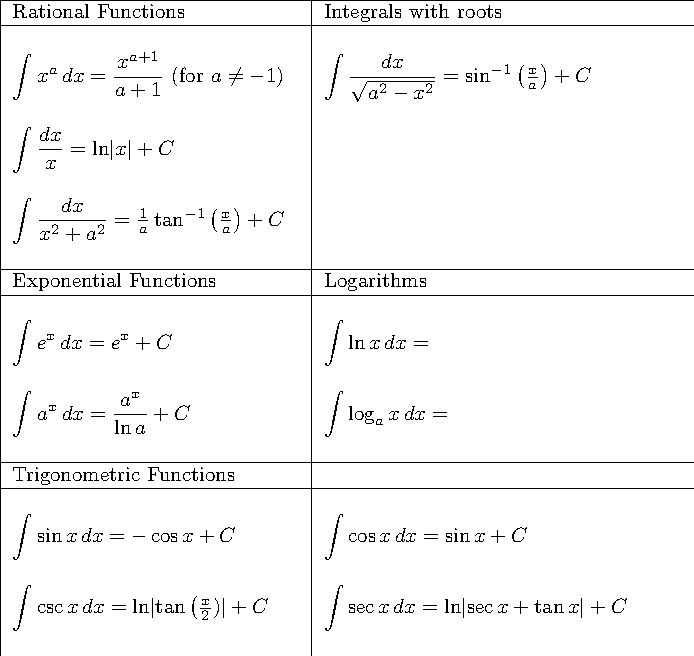
\includegraphics[width=\linewidth]{table.pdf}
\begin{tikzpicture}
  \node[scale=0.97]{
 \begin{tabular}{|m{1.2cm}|m{4.3cm}l||m{2.1cm}|m{4.3cm}l|}
 \hline
    $f(x)$\raisebox{0.5cm} & $\mathcal{L}\{f\}=\int_0^\infty e^{-sx}f(x)\, dx$\raisebox{0.5cm} & &
    \raisebox{0.5cm} & \raisebox{0.5cm} & \\[0.4cm] 
    \hline \hline
    $1$ & $\dfrac{1}{s}$\raisebox{0.6cm} & $s>0$ &
    $cf(x)\pm g(x)$ & $cF(s) \pm G(s)$\raisebox{0.4cm} & $s>max(a,b)$ \\[0.4cm]
    \hline
    $x^n$ & $\dfrac{n!}{s^{n+1}}$\raisebox{0.6cm} & $s>0$ & $e^{\alpha x}f(x)$ & $F(s-\alpha)$\raisebox{0.4cm} & $s>a+\alpha$ \\[0.4cm]
    \hline
    $e^{\alpha x}$ & $\dfrac{1}{s-\alpha}$\raisebox{0.6cm} & $s>\alpha$ &
    $x^n f(x)$ & $(-1)^n F^{(n)}(s)$\raisebox{0.4cm} & $s>a$ \\[0.4cm]
    \hline
    $\sin \beta x$ & $\dfrac{\beta}{s^2+\beta^2}$\raisebox{0.6cm} & $s>0$ & $f'(x)$ & $s F(s) -f(0)$\raisebox{0.4cm} & \\[0.4cm]
    \hline
    $\cos \beta x$ & $\dfrac{s}{s^2+\beta^2}$\raisebox{0.6cm} & $s>0$ &$f''(x)$\raisebox{0.4cm} & $s^2F(s) - sf(0)  - f'(0)$ & \\[0.4cm]
    \hline
    \end{tabular} };
    \end{tikzpicture}
\end{center}

\begin{itemize}
\item The slope of the tangent line to the curve at $(x_0,y_0)$ is $f'(x_0)$.
\item The slope of the normal line to the cure at $(x_0,y_0)$ is $-1/f'(x_0)$.
\item The equation of the tangent line at $(x_0,y_0)$ is $y-y_0=y'(x-x_0)$.
\item The equation of the normal line at $(x_0,y_0)$ is $y-y_0 = (x_0-x)/f'(x_0)$.
\item The $x$--intercept of the tangent is $x_0-f(x_0)/f'(x_0)$.
\item The $y$--intercept of the tangent is $f(x_0)-x_0 f'(x_0)$.
\item The $x$--intercept of the normal is $x_0+f(x_0)f'(x_0)$.
\item The $y$--intercept of the normal is $f(x_0)+x_0/f'(x_0)$.
\item The length of the tangent between $(x_0,y_0)$ and the $x$--axis is $\lvert y_0 \rvert\sqrt{1+1/f'(x_0)^2}$.
\item The length of the tangent between $(x_0,y_0)$ and the $y$--axis is $\lvert x_0 \rvert\sqrt{1+f'(x_0)^2}$.
\item The length of the normal between $(x_0,y_0)$ and the $x$--axis is $\lvert y_0 \rvert\sqrt{1+f'(x_0)^2}$.
\item The length of the normal between $(x_0,y_0)$ and the $y$--axis is $\lvert x_0 \rvert \sqrt{1+1/f'(x_0)^2}$.
\item The length of the subtangent is $\lvert f(x_0)/f'(x_0) \rvert$.
\item The length of the subnormal is $\lvert f(x_0) f'(x_0) \rvert$.
\end{itemize}



\end{document}
